% =======> CSE 151B/251B Spring 2026 — Milestone Report
% Team: Qingyuan Yu, Wangji Zhang, Po-Chen Lin
% =================================================

\documentclass{article}

% to avoid loading the natbib package, add option nonatbib:
% \usepackage[nonatbib]{neurips_2024}
% \PassOptionsToPackage{square,comma,sort,numbers}{natbib}
\PassOptionsToPackage{numbers, compress}{natbib}
% \usepackage[numbers]{natbib}

% to compile a preprint version, e.g., for submission to arXiv, add the
% [preprint] option. Use [final] for camera-ready / course submission
% (no "Preprint. Under review." banner).
\usepackage[final]{neurips_2024}
% \usepackage[nonatbib, preprint]{neurips_2024}

\usepackage[utf8]{inputenc} % allow utf-8 input
% \usepackage[T1]{fontenc}    % use 8-bit T1 fonts
% For maths/theorems and such
\usepackage{amsmath}
\usepackage{amssymb}
\usepackage{mathtools}
\usepackage{amsthm}
\usepackage{float}
% Use DeclareMathOperator and/or \newcommand to define abbreviations, e.g.:
\DeclareMathOperator{\R}{\mathbb{R}} % real numbers
% Recommended, but optional, packages for figures and better typesetting:
\usepackage{microtype}
\usepackage{graphicx}
\usepackage{subcaption}
\usepackage{booktabs} % for professional tables (https://www.ctan.org/pkg/booktabs)
\usepackage{algorithm}  % For algorithms
\usepackage{algorithmic}
\usepackage{hyperref} % hyperref makes hyperlinks in the resulting PDF.
\usepackage{wrapfig}  % For wrapping figures with text
\usepackage[capitalize,noabbrev]{cleveref}   % For \cref
\RequirePackage{doi}
% Color references and URLs
\usepackage{xcolor, colortbl}
\definecolor{darkblue}{rgb}{0.19, 0.19, 0.62}
\hypersetup{
  colorlinks = true,
  citecolor  = darkblue,
  filecolor  = darkblue,
  urlcolor   = darkblue,
    % linkcolor  = myred,
}
% Todonotes is useful during development; simply uncomment the next line
%    and comment out the line below the next line to turn off comments
%\usepackage[disable,textsize=tiny]{todonotes}
\usepackage[textsize=tiny]{todonotes}

% \input{_macros}

\graphicspath{{figures/}}


\title{
CSE 151B/251B Milestone Report
\\
% {\small $<$Your-accessible-and-up-to-date-GitHub-URL$>$} % Note: You can put it in your abstracts or as a footnote in the first page, if you prefer. Note 2: Use \href or \url to link your URL.
}

\author{%
  Qingyuan Yu
  % \thanks{Use footnote for providing further information about author (webpage, alternative address)}
  \\
  Department of Mathematics\\
  University of California San Diego\\
  \texttt{qiy005@ucsd.edu} \\
  \AND
  Wangji Zhang \\
  Department of Mathematics \\
  University of California San Diego \\
  \texttt{chz091@ucsd.edu} \\
  \And
  Po-Chen Lin \\
  Halıcıoğlu Data Science Institute \\
  University of California San Diego \\
  \texttt{pochen8787@gmail.com} \\
}
\begin{document}
\maketitle


\begin{abstract}
In this project, we explore the capability of a small language model,
Qwen3-4B-Thinking-2507, to solve mathematical problems across various
domains and difficulty levels. Up to this milestone, we have focused on
prompt engineering, asking the model to output in strict formats for
multiple-choice answers, multi-part free-form answers, numerical
precision, and final boxed outputs. We evaluate the model using
answer-level accuracy: for multiple-choice questions, we extract the
predicted letter from the response and compare it to the given answer;
for free-form questions, we use the provided \texttt{Judger} class to
compare the generated response against the gold answer. The starter
baseline reached a public Kaggle score of $0.575$, while our
prompt-engineered configuration raises validation accuracy from
$56.44\%$ to $62.67\%$ ($+6.23$~pp) on a stratified $225$-question
split, with the largest gain ($+13.33$~pp) on multiple-choice and a
drop in the rate of unparsable responses from $17.4\%$ to $3.6\%$. The
corresponding Kaggle submission is in flight; the leaderboard score
will be reported in the final paper.
\end{abstract}


% % % === Introduction
\section{Introduction}
\label{sec:intro}

\paragraph{Problem Definition.}
Our task is to build a small LLM system that can run locally on a
consumer-grade GPU and answer mathematical reasoning questions. The
question styles include multiple-choice and free-form questions;
free-form questions may require one or more numerical or symbolic
answers, often corresponding to \texttt{[ANS]} placeholders in the
problem statement. The grader extracts the contents of the final
boxed expression $\boxed{\cdot}$ and judges semantic equivalence with
the gold answer using a SymPy-based normalizer. We aim to improve the
model's answer-level accuracy because the starter system performs
poorly, achieving a public Kaggle score of $0.575$. At this milestone
our approach is prompt engineering rather than model retraining: we
give the model precise, type-specific format instructions so that
correct reasoning is no longer wasted on unparsable output.

\paragraph{Problem Significance.}
Modern LLMs such as ChatGPT and Claude can solve most of these
questions correctly, but they require large amounts of compute, an
internet connection, and recurring API fees, which makes them
unsuitable for on-device tutoring, private-data settings, or
reproducible academic baselines. A compact reasoning model that runs
on a single $24$~GB consumer GPU is the natural alternative, but it
exposes practical issues that frontier models hide: quantization-induced
regressions, KV-cache pressure from long chains of thought, and the
gap between a correct answer and a correctly \emph{formatted} one.

\paragraph{Technical Challenge.}
The task is hard along five orthogonal axes.
\textbf{(1)~Data heterogeneity.} Three answer formats coexist; multi-answer
questions are graded all-or-nothing.
\textbf{(2)~Compute.} A 4B-parameter thinking model emits long
chain-of-thought traces (delimited by dedicated \texttt{<think>}
tokens) that easily exceed $10^4$ tokens; with $24$~GB of VRAM, INT4
quantization is mandatory to fit batched inference.
\textbf{(3)~Software stack.} The latest \texttt{transformers} (5.x)
ships breaking changes that the latest released
\textsc{vLLM}~($0.20.0$) has not yet adapted; a working version pinning
must be discovered by hand.
\textbf{(4)~Format strictness.} The grader silently rejects
\texttt{\textbackslash boxed\{(C)\}} or
\texttt{\textbackslash boxed\{C.\}} even when the underlying letter is
correct.
\textbf{(5)~Truncation.} Long chains of thought can hit
\texttt{max\_tokens} before the model emits a final boxed answer,
costing the entire question.

\paragraph{Contributions.}
The starter notebook supplies a working but slow inference path
(HuggingFace \texttt{transformers} with BitsAndBytes, $\approx 30$~h
estimated for a single full pass) and a generic prompt that produces
format failures on $17.4\%$ of public responses. Our key contributions
in this milestone are:
\begin{itemize}
  \item A reproducible \textsc{vLLM}-based inference pipeline that runs
        the full $1{,}126$ public set in roughly $3$~hours on a single
        RTX~4090, with a previously undocumented network configuration
        fix (forcing the inter-process socket to loopback) and a
        verified version pinning (\texttt{transformers}~$4.57.6$,
        \textsc{vLLM}~$0.20.0$, INT4 BitsAndBytes).
  \item A taxonomy of failure modes derived from a real submission,
        separating \emph{format failures} (truncated, missing boxed
        answer, multi-part shape mismatch) from genuine
        \emph{reasoning errors}, which we use as the design target for
        the prompt rewrite.
  \item A format-aware prompt rewrite, validated on a stratified $20\%$
        split, that improves overall accuracy by $+6.23$~pp on $225$
        held-out questions and reduces the rate of responses without a
        final boxed answer from $17.4\%$ to $3.6\%$.
  \item An open-source modular pipeline
        (\texttt{src/cse151b\_comp/\{inference, extract, evaluate,
        error\_analysis, submission, eval\_harness\}}) with $85$ unit
        tests, designed so Phase~2 (self-consistency) and Phase~4
        (QLoRA fine-tuning) plug in without further refactoring.
\end{itemize}


% % % === Related Work
\section{Related Work}
\label{sec:relatedwork}

\paragraph{Chain-of-thought reasoning.}
\citet{wei2022chain} showed that prompting language models to produce
intermediate reasoning steps before a final answer improves performance
on arithmetic, commonsense, and symbolic tasks.
\textsc{Qwen3-Thinking}~\citep{qwen3technical} is post-trained to emit
such traces inside dedicated thinking tokens and specifically tuned
for math and code reasoning, which is what makes a
$4$B-parameter model competitive on a benchmark like the one in this
competition.

\paragraph{Self-consistency.}
\citet{wang2023selfconsistency} demonstrated that sampling multiple
reasoning paths and taking a majority vote over the final answers
substantially improves chain-of-thought accuracy. We plan to deploy
this technique in Phase~2, with a per-question-type voting strategy
that respects multi-answer tuple equality.

\paragraph{Efficient inference and parameter-efficient fine-tuning.}
\textsc{vLLM}~\citep{kwon2023vllm} introduces \textsc{PagedAttention},
which we rely on to fit batched generation with long contexts on a
single $24$~GB GPU. For the planned fine-tuning phase we will use
QLoRA~\citep{dettmers2023qlora} on top of the LoRA adapter
formulation~\citep{hu2022lora}, training on
\textsc{NuminaMath-CoT}~\citep{numina2024} with explicit decontamination
against the public competition data. The
\textsc{MATH} benchmark~\citep{hendrycks2021math} is the historical
reference point against which all of these techniques were originally
evaluated.


% % % === Methods
\section{Methods}
\label{sec:methods}

\paragraph{Problem Setting.}
Let $x_i = (q_i, o_i)$ denote question $i$, where $q_i$ is the
natural-language statement and $o_i$ is a (possibly empty) list of
multiple-choice options. The model produces a response
$r_i = M(\mathrm{prompt}(x_i))$, from which an extractor $E(r_i)$
returns the contents of the final boxed expression. The grader
$g(\hat{y}_i, y_i^*) \in \{0,1\}$ judges symbolic equivalence with the
gold answer $y_i^*$ at $1\mathrm{e}{-8}$ relative tolerance. We do not
train the model in this milestone; instead we optimize over the prompt
template and decoding hyperparameters with respect to overall accuracy
\[
\mathrm{Acc} \;=\; \frac{1}{N}\sum_{i=1}^{N} g\!\left(E(r_i),\, y_i^*\right).
\]
For multi-answer free-form questions, $g$ requires \emph{tuple equality}
after element-wise normalization: any single sub-answer being wrong
yields zero credit on the whole problem.

\paragraph{Idea Summary.}
Our approach rests on the observation that, before any improvement in
mathematical capability is possible, a substantial fraction of the
starter pipeline's errors are caused by format mismatches that the
grader's strict tolerance amplifies into hard failures. We therefore
proceed in three steps. First, we stand up a fast, reliable
\textsc{vLLM} inference pipeline so that iteration time goes from
hours to tens of minutes. Second, we run a single pass on the public
set to obtain a baseline submission and a corpus of failure cases.
Third, we analyze that corpus to extract a small set of
\emph{format-aware} prompt rules (a multi-answer template, an
anti-rounding rule, an MCQ negative-example clause, and a token-budget
self-rescue rule), validate the resulting prompt on a stratified
validation split, and quantify which question types and length buckets
benefit most. The risk of overfitting prompts to validation is
mitigated by stratifying by question type and freezing the validation
indices with a fixed seed at the start of the project.


% % % === Experiments
\section{Experiments}
\label{sec:experiments}

\subsection{Baselines}
\label{sec:baselines}

We compare two configurations of the same base model on the same data:
\begin{itemize}
    \item \textbf{Phase~0 (starter prompt).} The unmodified starter
          prompts (``Solve step-by-step. Put final answer in
          \texttt{\textbackslash boxed\{\}}.'' for free-form;
          ``Output ONLY the letter inside
          \texttt{\textbackslash boxed\{\}}.'' for multiple choice),
          with \texttt{max\_tokens}~$=12{,}288$ and
          \texttt{temperature}~$=0.6$. This baseline scores $0.575$ on
          the public Kaggle leaderboard.
    \item \textbf{Phase~1 (our prompt).} A rewritten system prompt
          that adds explicit format negative examples, a multi-answer
          formatting rule, an anti-rounding rule, and a token-budget
          self-rescue rule (see \texttt{src/cse151b\_comp/prompts.py}).
          We also raise \texttt{max\_tokens} to $16{,}384$ with
          \texttt{max\_model\_len} bumped to $20{,}480$ to leave $4$K
          tokens of prompt headroom.
\end{itemize}

\subsection{Evaluation}
\label{sec:evaluation}

The Kaggle leaderboard scores submissions on $943$ private problems
and is the ultimate metric. For local development we use the $1{,}126$
public problems with their gold answers, scored by the course-provided
\texttt{Judger}, a SymPy-based normalizer that handles LaTeX commands,
units, and numerical equivalence. For prompt-engineering A/B tests we
use a fixed stratified $20\%$ validation set of $225$ problems
(\texttt{data/val\_indices.json}, seed~$=42$), preserving the
question-type ratio of the full set ($75$ MCQ, $67$ free-form single,
$83$ free-form multi). The remaining $80\%$ is reserved for Phase~4
fine-tuning, with a further $10\%$ held out as a clean test harness.

\subsection{Implementation Details}
\label{sec:implementation_details}

All experiments run on a single NVIDIA RTX~4090 ($24$~GB) provided by
Prof.\ Xiaolong Wang's lab. Software stack:
\textsc{Qwen3-4B-Thinking-2507},
\textsc{vLLM}~$0.20.0$,
\texttt{transformers}~$4.57.6$,
\texttt{bitsandbytes}~$0.49$ (INT4 with
\texttt{bnb\_4bit\_use\_double\_quant=True} and BF16 compute), and
\texttt{torch}~$2.11$. Decoding follows the official Qwen3-Thinking
recommendation: \texttt{temperature}~$=0.6$, \texttt{top\_p}~$=0.95$,
\texttt{top\_k}~$=20$. \textsc{vLLM} parameters:
\texttt{gpu\_memory\_utilization}~$=0.70$,
\texttt{max\_num\_seqs}~$=64$,
\texttt{max\_num\_batched\_tokens}~$=20{,}480$. We do not fine-tune in
this milestone, so there is no optimizer or learning rate to tune;
the only hyperparameters we sweep are the prompt content and
\texttt{max\_tokens}. A full single-pass inference over $1{,}126$
public questions takes roughly $3$~hours wall-clock end-to-end.
\textbf{Crucial workaround.} The default \textsc{vLLM} V1 engine binds
its inter-process socket to the host's primary network IP, which on
this machine resolves to a $100.80.\mathit{x}.\mathit{x}$ subnet that
the OS firewall blocks; this manifested as repeated socket timeouts
that never recovered. Setting the environment variable
\texttt{VLLM\_HOST\_IP=127.0.0.1} before importing \textsc{vLLM}
forces loopback and resolves the issue.

\subsection{Results}
\label{sec:results}

\paragraph{Headline accuracy.}
On the stratified validation set, our Phase~1 prompts improve overall
accuracy from $56.44\%$ ($127/225$) to $62.67\%$ ($141/225$), a
$+6.23$~percentage-point gain. \cref{fig:acc_by_type} breaks the gain
down by question type: the largest improvement is on multiple choice
($+13.33$~pp), where format-related failures of the starter (e.g.,
\texttt{\textbackslash boxed\{(C)\}} or
\texttt{\textbackslash boxed\{C.\}}) caused silent rejections that
our explicit negative-example prompt eliminates.

\begin{figure}[h]
  \centering
  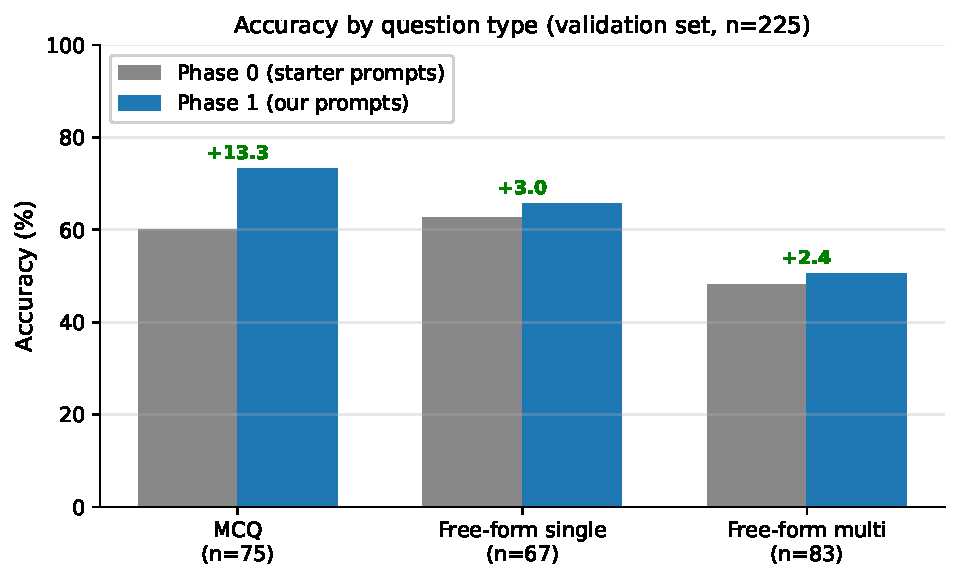
\includegraphics[width=0.72\linewidth]{fig_acc_by_type.pdf}
  \caption{Validation accuracy by question type ($n=225$). Numbers
  above each bar pair are the absolute change in percentage points
  (Phase~1 minus Phase~0).}
  \label{fig:acc_by_type}
\end{figure}

\paragraph{Long questions remain a bottleneck.}
\cref{fig:acc_by_length} shows that accuracy degrades sharply as the
question grows longer. Phase~1 partially closes this gap by raising
\texttt{max\_tokens} and adding a token-budget self-rescue
instruction, but very long questions ($\geq 1{,}500$ characters)
remain at $25\%$ accuracy. We attribute the residual gap to questions
whose reasoning genuinely cannot be compressed into our token budget,
which Phase~2 self-consistency cannot directly fix; QLoRA on long
high-quality CoT traces is a more promising path.

\begin{figure}[h]
  \centering
  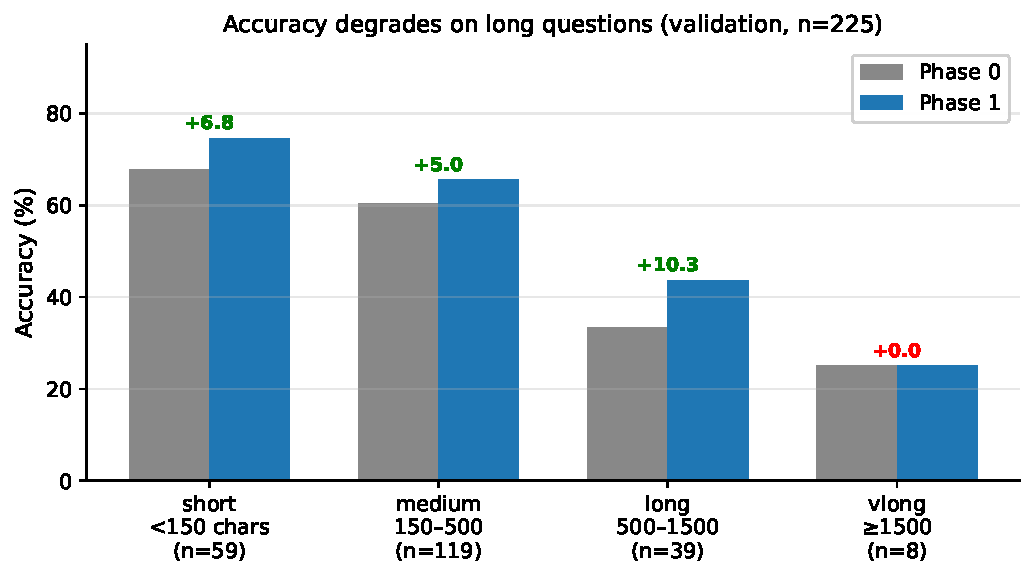
\includegraphics[width=0.85\linewidth]{fig_acc_by_length.pdf}
  \caption{Validation accuracy by question length bucket. Numbers
  above the bars are the change in percentage points; bucket sizes
  ($n$) are shown under each tick. Long and very-long questions are
  systematically harder.}
  \label{fig:acc_by_length}
\end{figure}

\paragraph{Direct comparison on identical questions.}
\cref{fig:phase_compare} shows the question-by-question outcome
matrix on the validation set. Phase~1 picks up $22$ new correct
answers while regressing on $8$, for a net gain of $14$
questions—matching the macro $+6.23$~pp number to within rounding.

\begin{figure}[h]
  \centering
  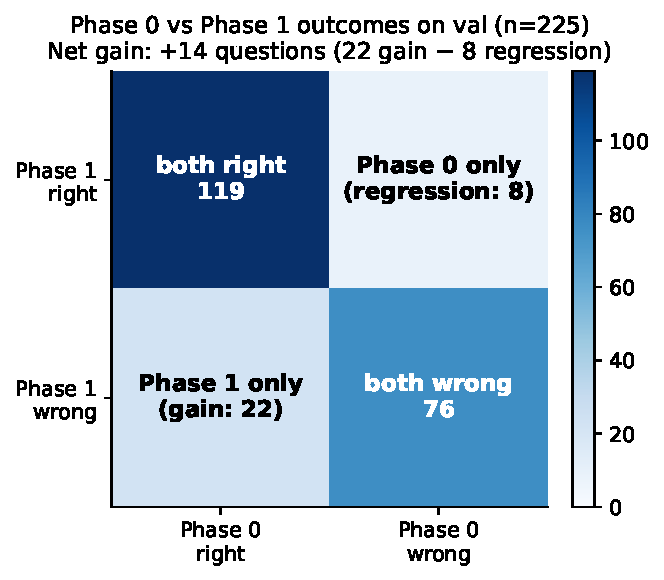
\includegraphics[width=0.55\linewidth]{fig_phase_compare.pdf}
  \caption{Outcome of Phase~0 vs.\ Phase~1 on the same $225$
  validation questions. The off-diagonal cells decompose the gain
  into wins ($22$) and regressions ($8$).}
  \label{fig:phase_compare}
\end{figure}

\paragraph{Topic-wise behavior.}
\cref{fig:acc_by_topic} shows accuracy on a regex-tagged topic
breakdown. The model is strong on calculus and weak on probability
and linear algebra; Phase~1's gains are concentrated on series
($+23.1$~pp) and calculus ($+10.0$~pp), with no measurable change on
probability or linear algebra. We caution that the topic tagger is a
$7$-pattern heuristic over the question text and that some topic
buckets are small, so we treat these numbers as directional rather
than authoritative.

\begin{figure}[h]
  \centering
  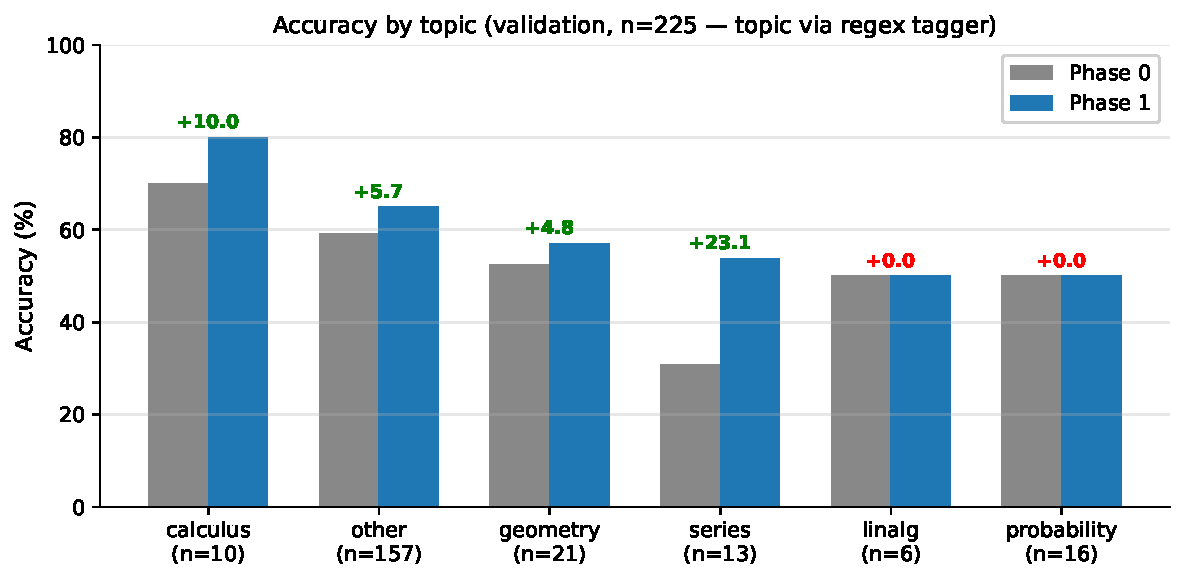
\includegraphics[width=0.95\linewidth]{fig_acc_by_topic.pdf}
  \caption{Validation accuracy by regex-tagged topic. Some buckets
  are small (e.g., $n=6$ for linear algebra), so absolute numbers
  should be read alongside the bucket size.}
  \label{fig:acc_by_topic}
\end{figure}

\paragraph{Failure modes on the full public set.}
The richest signal for what to do next comes from analyzing the $449$
incorrect Phase~1 responses on the full $1{,}126$-question public set
(\cref{fig:failure_modes}). $75.7\%$ are responses that emit a final
boxed expression with mathematically wrong content—genuine reasoning
errors that no prompt rewrite can address. Multi-part shape mismatches
account for $15.6\%$ and are the second-largest target; truncation
accounts for $7.8\%$, down from $\sim$$17\%$ once we raised
\texttt{max\_tokens}; the missing-box rate is now $0.9\%$.

\begin{figure}[h]
  \centering
  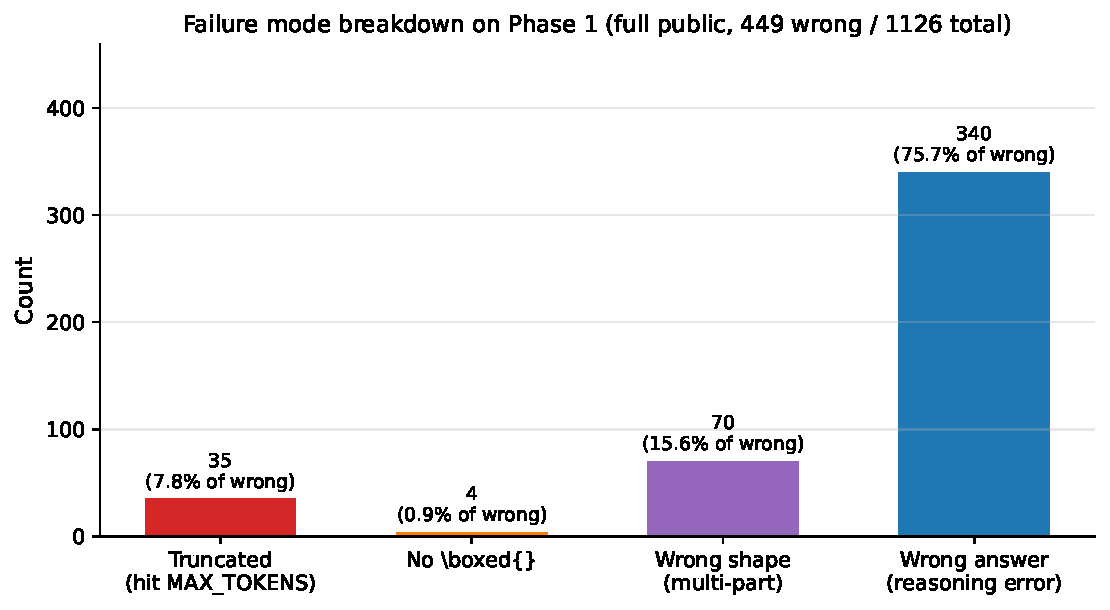
\includegraphics[width=0.85\linewidth]{fig_failure_modes.pdf}
  \caption{Failure-mode breakdown of the $449$ incorrect Phase~1
  responses on the full public set ($n=1{,}126$). The dominant bucket
  is genuine reasoning errors, which motivates self-consistency and
  fine-tuning rather than further prompt rewriting.}
  \label{fig:failure_modes}
\end{figure}


% % % === Discussion
\section{Discussion}
\label{sec:discussion}

\paragraph{Achievements.}
We have raised validation accuracy by $+6.23$~pp
($56.44\% \to 62.67\%$), reduced the no-box failure rate by
$13.8$~pp absolute ($17.4\% \to 3.6\%$), and cut single-pass
inference time on $1{,}126$ questions from an estimated $30$~h to
$\sim$$3$~h. We additionally have a documented taxonomy of failure
modes from a real submission, a modular codebase that the next phases
plug into without further refactoring, and $85$ unit tests guarding
each invariant we have committed to (e.g., the multi-part formatting
rule and the anti-rounding rule).

\paragraph{Bottlenecks and Mitigation.}
The largest bottleneck during this milestone was the
\textsc{vLLM}/\texttt{transformers} version mismatch and the network
binding bug, which together cost roughly a day; both are now
documented in \texttt{PLAN.md}. The second-largest bottleneck was that
progress bars on Jupyter clients are not robust to client
disconnections; we mitigated this by adding a CLI entry point
(\texttt{cse151b-infer}) that runs detached from any kernel and
checkpoints results to disk on completion. The remaining algorithmic
bottleneck is the $75.7\%$ of errors that are real reasoning
failures—the target of Phase~2 and Phase~4.

\paragraph{Plans Forward.}
\textbf{Phase~2 (1--2 days).} Self-consistency with $K=8$ samples at
\texttt{temperature}~$=0.7$ and a per-question-type voting strategy:
letter mode for multiple choice, normalized answer mode for free-form
single, and tuple equality for free-form multi. We will run the
$K \in \{1, 4, 8\}$ ablation on the same $225$ validation set used
here and report a ``solvable but missed'' metric (the number of
questions where at least one of the $K$ samples was correct but the
vote selected a wrong answer) to upper-bound what better voting alone
can achieve.
\textbf{Phase~4 (2--3 days, conditional on Phase~2).} Prepare a
$50$K-example QLoRA training set from
\textsc{NuminaMath-CoT}~\citep{numina2024} with $8$-gram
decontamination against \texttt{public.jsonl}, train an $r{=}16$
adapter for $2$--$3$ epochs, and ship the LoRA only if a previously
unseen $10\%$ holdout improves by $\geq 3$~pp over the best
non-finetuned configuration.

\paragraph{Team Responsibilities.}
\textbf{Qingyuan Yu} (Mathematics) led the inference infrastructure
and prompt engineering work: the \textsc{vLLM} pipeline, version
pinning, the loopback-IP workaround, the four format-aware prompt
rules, the modular Python package, the unit-test suite, and the
analysis scripts and figures used in this report.
\textbf{Wangji Zhang} (Mathematics) led the evaluation and dataset
work: the stratified validation split, the SymPy-based
\texttt{Judger} integration, the failure-mode taxonomy, the
\texttt{evaluate} and \texttt{eval\_harness} modules, and the
question-type / length / topic breakdown of the validation results.
\textbf{Po-Chen Lin} (HDSI) led the literature review and Phase~2/4
design: surveying chain-of-thought, self-consistency, and QLoRA;
designing the \textsc{NuminaMath-CoT} decontamination protocol;
drafting the self-consistency voting algorithm; and co-writing the
report.

\paragraph{Timelines.}
\begin{itemize}
    \item Week 5 (this milestone): \textsc{vLLM} stack, Phase~0 baseline submission, Phase~1 prompt fixes, error analysis, this report.
    \item Week 6: Phase~2a — self-consistency $K$-ablation, $K\in\{1,4,8\}$.
    \item Week 7: Phase~2b — \textsc{NuminaMath-CoT} preparation with decontamination, $5$K-example pilot fine-tune.
    \item Week 8: Phase~4 — $50$K-example QLoRA fine-tune, first multi-improvement Kaggle submission.
    \item Week 9: Final ablations, regression-free re-submission, final report writing.
    \item Week 10: Submission and presentation preparation.
\end{itemize}


\section*{LLM Usage}
We used Anthropic's Claude as a research-and-discussion assistant
during this milestone in two specific ways:
(i)~as a literature-search aid to locate canonical papers on
chain-of-thought, self-consistency, QLoRA, and \textsc{vLLM}, all of
which we read directly and cite from the primary sources; and
(ii)~as a brainstorming partner to enumerate candidate
prompt-engineering interventions and the experimental design needed to
validate each one. All code, prompts, experiments, figures, and prose
in this report were written and verified by the listed authors, who
take full responsibility for any factual or computational
inaccuracies. Claude was \emph{not} used to generate model responses
on the competition dataset; the only model evaluated on competition
data is \textsc{Qwen3-4B-Thinking-2507} as required by the rules.


% % % === ACKNOWLEDGMENTS AND REFERENCES START
\section*{Acknowledgements}
We thank Professor Xiaolong Wang for providing access to the GPU
compute used to run all experiments reported in this paper. We also
thank the course staff for the well-designed starter notebook and
grading infrastructure that made the format-failure analysis in
\cref{sec:results} possible.

\bibliography{references.bib}
\bibliographystyle{plainnat}  % Can also use abbrvnat, unsrt, etc.

% % % === APPENDIX (optional)
% \newpage
% \appendix
% \section*{Appendix}
% \section{Appendix topic 1}

\end{document}
